\chapter{Desarrollo e implementación}

En este capítulo se abordará cómo se ha llevado a cabo el proceso de implementación del proyecto, partiendo desde la preparación del entorno para la realización de ataques y posterior generación del \textit{dataset} de logs, siguiendo por cómo se ha preprocesado dicho \textit{dataset} y otros extraídos de fuentes públicas para la comparación de resultados, y finalmente la implementación de las distintas técnicas de \textit{clustering} y la selección de métricas para evaluar los resultados obtenidos.

% ********************************************************************

\section{Simulación de ataques y generación de logs}

A continuación, se verá en detalle cómo se han desarrollado los conjuntos de datos de \textit{logs} de Linux. En primer lugar, se ha realizado un \textit{dataset} de manera totalmente manual, y finalmente se ha hecho uso de un \gls{LLM} para la generación de un \textit{dataset} sintético y ya estructurado que simula dichos \textit{logs}.

\vspace{-3mm}

\subsection{Dataset Manual}

Como se ha comentado en capítulos anteriores, para la simulación de ataques se hará uso del framework de \gls{CALDERA} \cite{caldera}. Antes de mostrar este proceso paso a paso, es importante recalcar que toda la implementación de esta sección se hará sobre el sistema operativo Kali Linux 6.5.0-kali3-amd64 Debian \gls{GNU}/Linux  tal y como se indica en la Figura \ref{fig:uname-kali}, aunque podría ser emulado de forma equivalente en otras distribuciones de Linux.

\begin{figure}[H]
    \centering
    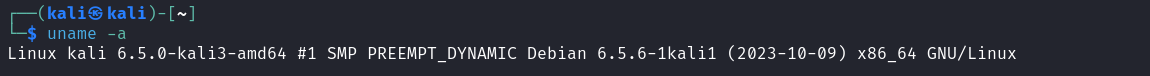
\includegraphics[width=1\linewidth]{imagenes/uname-kali.png}
    \caption{Distribución de Linux utilizada para la Simulación de ataques}
    \label{fig:uname-kali}
\end{figure}

Sobre este, colgarán 2 contenedores Docker con la distribución de Ubuntu Server que serán utilizados como máquinas víctima para llevar a cabo los ataques. Además del uso de este \textit{framework} de MITRE, se hará uso de otros servicios como Syslog, \gls{SFTP} o \gls{SSH}. La máquina Kali actuará como servidor central y por tanto los \textit{logs} de las máquinas que son objeto de ataque tendrán un flujo de salida hacia este, de modo que a través de la configuración de Syslog se irá formando un fichero \.log que dará forma al \textit{dataset} en formato \textit{raw}. Al mismo tiempo, por simplicidad, actuará como máquina atacante dentro de la misma subred que simula la infraestructura empresarial.

\vspace{-2mm}

\subsubsection*{Configuración del Servidor Syslog y Máquinas Víctima}

Con el fin de llevar a cabo la emulación de ataques sobre los contenedores y que los eventos generados se almacenaran en un único fichero, fue necesario diseñar la arquitectura del entorno, incluyendo los servicios utilizados,  ficheros de configuración necesarios, así como el orden a seguir para preparación. En primer lugar, se definió la arquitectura de modo que las máquinas involucradas fueran:

\begin{table}[H]
\footnotesize
\begin{tabularx}{\linewidth}{|l|X|}
    \hline
    \rowcolor{graylight}\texttt{Máquina} & \texttt{Descripción} \\
    \hline
    \texttt{KALI\_LINUX} & Máquina principal con el framework de \gls{CALDERA} instalado y servidor de Syslog para monitorizar los logs. \newline Virtualizado con Oracle \gls{VM} VirtualBox. \\
    \hline
    \texttt{UBUNTU\_SERVER\_1} & Primera máquina víctima, contenedor de Docker levantado sobre máquina Kali. \\
    \hline
    \texttt{UBUNTU\_SERVER\_1} & Segunda máquina víctima, contenedor de Docker levantado sobre máquina Kali. \\
    \hline
\end{tabularx}
\caption{Máquinas utilizadas para la simulación de ataques y recolección de \textit{logs}}
\label{tab:machines}
\end{table}

Cada una de las máquinas reenviará el flujo de \textit{logs} al servidor de Syslog ubicado en la máquina Kali. De tal modo, será posible almacenar en un mismo fichero los \textit{logs} de cada una, como se ilustra en la Figura \ref{fig:entorno-ataques}.

\vspace{2mm}

\begin{figure}[H]
    \centering
    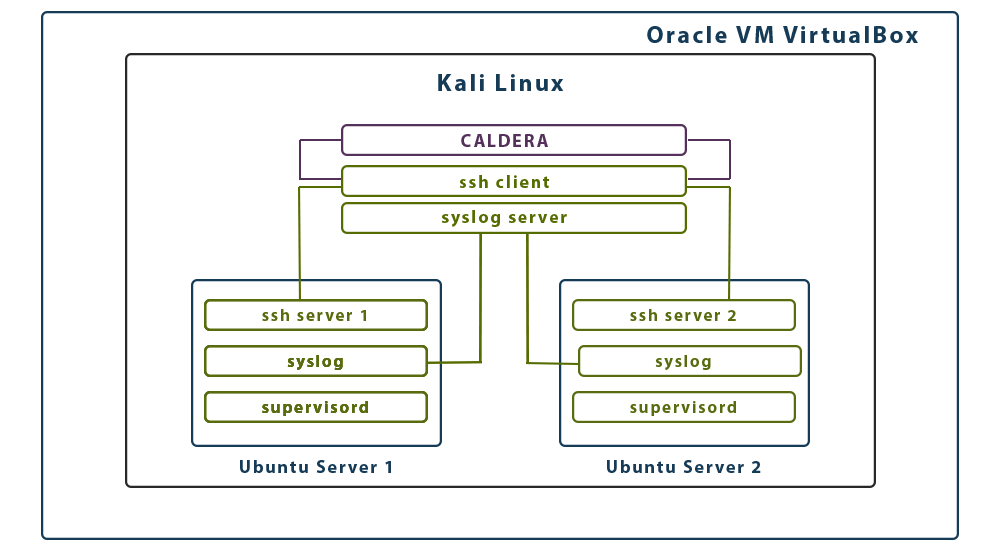
\includegraphics[width=1\linewidth]{imagenes/Enviromentv2.png}
    \caption{Arquitectura del entorno de simulación de ataques}
    \label{fig:entorno-ataques}
\end{figure}

\newpage

Se realizaron los siguientes pasos: \\

1. Acceder a la ruta donde se ubica el fichero Dockerfile y ejecutar el siguiente comando para construir la imagen \texttt{ubuntu-logger}:

\begin{mdframed}
\footnotesize
 \begin{minted}{docker}
docker build -t ubuntu-logger .
\end{minted}   
\end{mdframed}

2. Crear las máquinas a partir de la imagen generada:

\begin{mdframed}
\footnotesize
\begin{minted}{docker}
docker run -d --name ubuntu-logger-1 ubuntu-logger
docker run -d --name ubuntu-logger-2 ubuntu-logger
\end{minted}
\end{mdframed}

3. Iniciar una shell en ambas máquinas:

\begin{mdframed}
\footnotesize
\begin{minted}{docker}
docker exec -it ubuntu-logger-1 /bin/bash
docker exec -it ubuntu-logger-2 /bin/bash
\end{minted}
\end{mdframed}

Para construir las imágenes de los contenedores de Ubuntu Server \cite{ubuntu_server} se utilizó el siguiente fichero Dockerfile:

\begin{center}
\begin{mdframed}
\footnotesize
    \begin{minted}{docker}
# Se utiliza la imagen oficial de Ubuntu
FROM ubuntu:latest

# Evita preguntas al instalar paquetes
ARG DEBIAN_FRONTEND=noninteractive

# Actualiza los repositorios
RUN apt-get update
#Instala rsyslog, nano, iproute2, openssh-server y supervisor
RUN apt-get install -y rsyslog nano iproute2 curl openssh-server \
supervisor

# Configura rsyslog para enviar logs a máquina host y desactivar imklog
RUN sed -i 's/module(load="imklog")/#module(load="imklog")/' \
/etc/rsyslog.conf && echo '*.* @@172.17.0.1:514' >> /etc/rsyslog.conf

# Configura SSH para permitir acceso root con contraseña
RUN sed -i 's/#PermitRootLogin prohibit-password/PermitRootLogin yes/' \
/etc/ssh/sshd_config && echo 'root:root' | chpasswd

# Configuración de supervisord
COPY supervisord.conf /etc/supervisor/conf.d/supervisord.conf

# Expone los puertos necesarios para syslog y SSH
EXPOSE 514 22

# Configura supervisord como el comando principal
CMD ["/usr/bin/supervisord"]
    \end{minted}
\end{mdframed}
\end{center}

\newpage

A continuación, es necesario editar el fichero \texttt{supervisord.conf} en los contenedores. Este, utilizado para la configuración de  \texttt{supervisord}, gestiona los procesos del sistema, asegurando que los servicios definidos se inicien y mantengan en ejecución, concretamente \texttt{ssh} y \texttt{rsyslog}. 

\begin{center}
\begin{mdframed}
\footnotesize
    \begin{minted}{bash}
[supervisord]
nodaemon=true

[program:sshd]
command=/usr/sbin/sshd -D

[program:rsyslogd]
command=/usr/sbin/rsyslogd -n
    \end{minted}
\end{mdframed}
\end{center}

Por otro lado, el fichero de configuración \texttt{rsyslog.conf} utilizado en la máquina Kali Linux define cómo se manejan los registros de las máquinas Ubuntu Server 1 y Ubuntu Server 2. 

Este permite la recolección y almacenamiento de \textit{logs} provenientes de estas, que están dentro de la misma subred. Dicho fichero debe de tener activos los módulos de \gls{TCP} y \gls{UDP} para que la transferencia de \textit{logs} se realice correctamente:

\begin{center}
\begin{mdframed}
\footnotesize
    \begin{minted}{bash}
# /etc/rsyslog.conf configuration file for rsyslog

module(load="imuxsock")
module(load="imklog")

module(load="imudp")
input(type="imudp" port="514")

module(load="imtcp")
input(type="imtcp" port="514")

    \end{minted}
\end{mdframed}
\end{center}

Además, es necesario añadir la siguiente línea al final del fichero para que almacene todos los tipos de ficheros de \textit{log} en un único archivo \texttt{dataset-raw.log}:

\begin{center}
\footnotesize
\begin{mdframed}
    \begin{minted}{bash}
*.* /var/log/dataset-raw.log
    \end{minted}
\end{mdframed}
\end{center}

Finalmente, es necesario que el fichero \texttt{rsyslog.conf} de los contenedores tenga el siguiente contenido, para que se envíen los \textit{logs} a la máquina Kali:

\begin{center}
\begin{mdframed}
\footnotesize
    \begin{minted}{bash}
# /etc/rsyslog.conf configuration file for rsyslog

module(load="imuxsock") # provides support for local system logging
module(load="imklog" permitnonkernelfacility="on")

$IncludeConfig /etc/rsyslog.d/*.conf
    \end{minted}
\end{mdframed}
\end{center}


\newpage

Es necesario añadir al final del fichero las siguientes líneas:

\begin{center}
\begin{mdframed}
\footnotesize
    \begin{minted}{bash}
*.* @@172.17.0.1:514
cron,kern,mail,user,auth,authpriv.* @@172.17.0.1:514
    \end{minted}
\end{mdframed}
\end{center}

Estas especifican la redirección de los \textit{logs} generados en los contenedores hacia el servidor de syslog centralizado, en este caso, la máquina Kali Linux con la dirección \gls{IP} \texttt{172.17.0.1} a través del puerto \texttt{514}. 

La primera línea indica que todos los mensajes de \textit{log}, independientemente de su nivel de severidad o su origen, deben ser enviados al servidor central. Por otro lado, la segunda, refuerza esta configuración para logs específicos generados por las \textit{facilities} \ref{tab:syslog_facilities} \texttt{cron}, \texttt{kern}, \texttt{mail}, \texttt{user}, \texttt{auth}, y \texttt{authpriv}.

\subsubsection*{Simulación de Ataques con \gls{CALDERA}}

Una vez se ha instalado y configurado correctamente el \textit{framework} de \gls{CALDERA} siguiendo la documentación del Anexo \ref{caldera-conf}, puede llevarse a cabo la simulación de ataques sobre los contenedores \texttt{UBUNTU\_SERVER\_1} y \texttt{UBUNTU\_SERVER\_2}. Dentro de la interfaz web del \textit{framework},simplemente basta con acceder a la sección de operaciones y hacer click sobre el botón de \texttt{Start} para iniciar la operación. La principal ventaja de este \textit{framework} es que la interfaz proporciona una monitorización en tiempo real de la ejecución de las operaciones, de modo que puedan verse los resultados que van obteniéndose, así como el orden de las tácticas y técnicas empleadas en dicho proceso de ataque.

\begin{figure}[H]
    \centering
    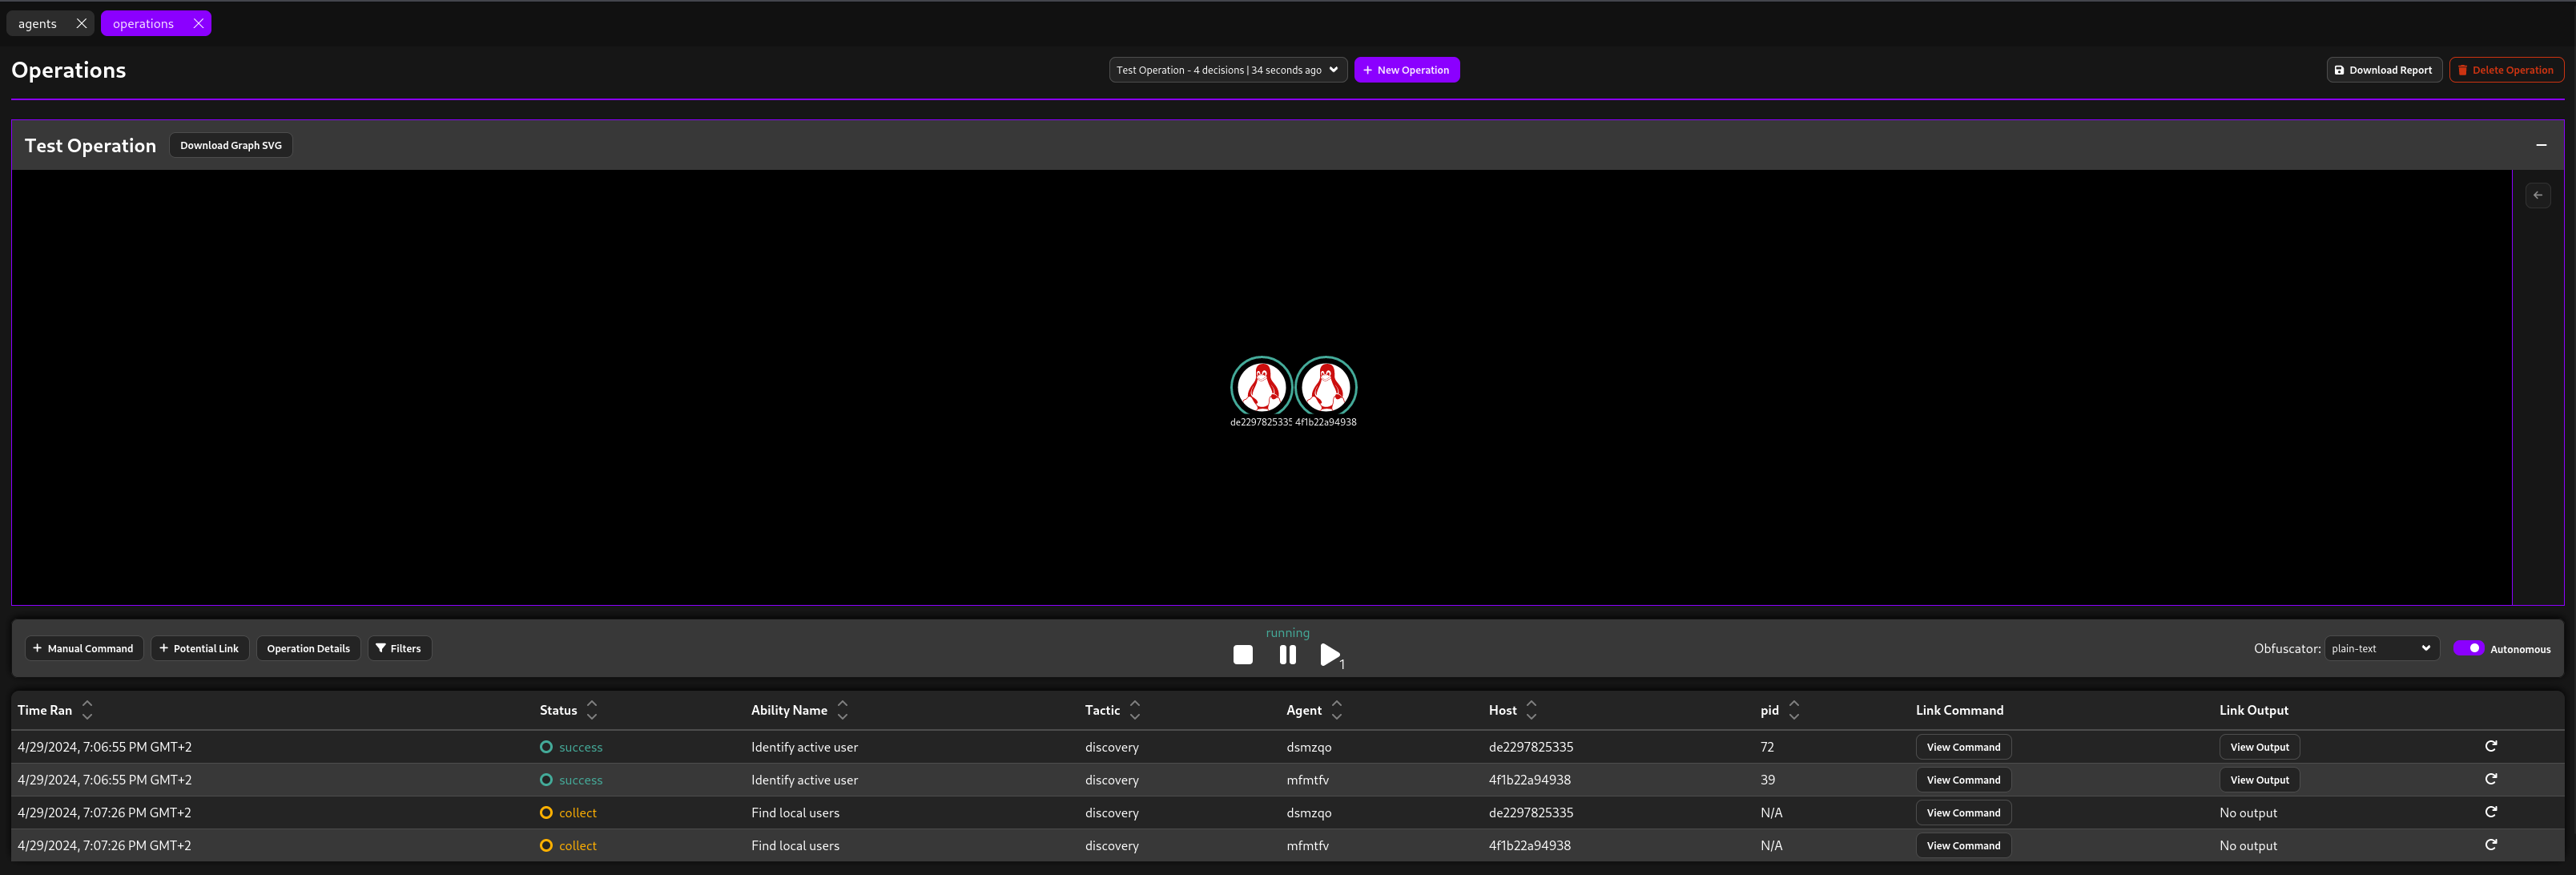
\includegraphics[width=1\linewidth]{imagenes/operation-start.png}
    \caption{Ejemplo de ejecución de una operación de Discovery con \gls{CALDERA}}
    \label{fig:operation-start}
\end{figure}

Tal y como se muestra en la Figura \ref{fig:operation-start}, el panel de operaciones una vez iniciado el ataque se divide en dos zonas. En primer lugar, la zona superior muestra las máquinas que están siendo atacadas y el tipo de sistema operativo de estas. En este caso son los dos contenedores de \texttt{Ubuntu Server}. En segundo lugar, la zona inferior detalla la información relativa al ataque, como es el tiempo de ejecución, el estado de la operación (p.e. \textit{success} o \textit{collect}), el nombre de la habilidad asociada, la táctica utilizada, el agente asociado al \textit{host}, el identificador del host, el \texttt{ID} del proceso e incluso el comando utilizado y su \textit{output} generado. 

Al mismo tiempo que se llevaban a cabo las operaciones, se fueron almacenando los eventos de \textit{logs} en las máquina víctima y enviándose de forma síncrona al servidor Syslog de la máquina \texttt{KALI\_LINUX}, como se muestra en la Figura \ref{fig:log-monitoring-syslog}. 

\begin{figure}[H]
    \centering
    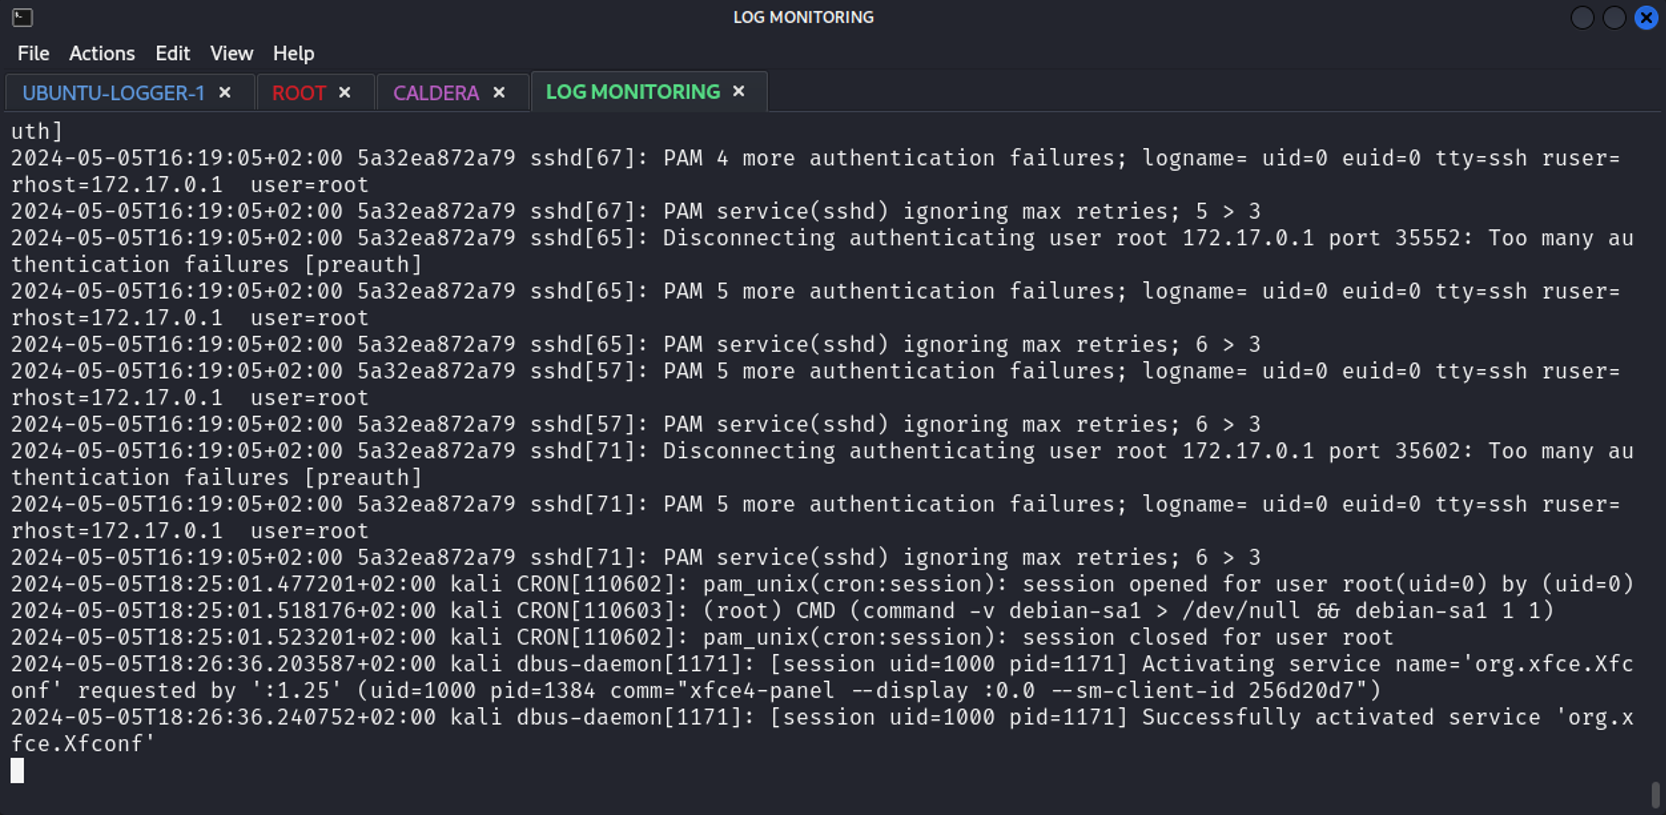
\includegraphics[width=1\linewidth]{imagenes/log-monitoring-syslog.png}
        \caption{Monitorización de \textit{logs} generados en máquinas víctima por operaciones}
    \label{fig:log-monitoring-syslog}
\end{figure}

\subsubsection*{Simulación de Ataques con otras herramientas}

Una vez efectuados los ataques en la infraestructura de red interna a través de \gls{CALDERA}, se llevó a cabo adicionalmente una serie de ataques adicionales a través de intentos de acceso externo mediante varias herramientas distintas indicadas anteriormente en \ref{adicional-tools}: \texttt{Metasploit} e \texttt{Hydra}. El proceso para cada una de ellas fue el siguiente: \\

En el caso de \texttt{Hydra}, se llevó a cabo un ataque por diccionario al servicio de \gls{SSH} como el mostrado en la Figura \ref{fig:hydra-ssh}, utilizando uno de los disponibles en la carpeta \texttt{/usr/share/wordlists/} de cualquier distribución \texttt{Kali}, en este caso el famoso diccionario \textit{Rockyou} \cite{kanta2022novel}. El comando utilizado fue:

\begin{center}
\begin{mdframed}
\scriptsize
    \begin{minted}{bash}
    hydra -l test-user -P /usr/share/wordlists/rockyou.txt.gz ssh://172.17.0.2
    \end{minted}
\end{mdframed}
\end{center}

\begin{figure}[H]
        \centering
        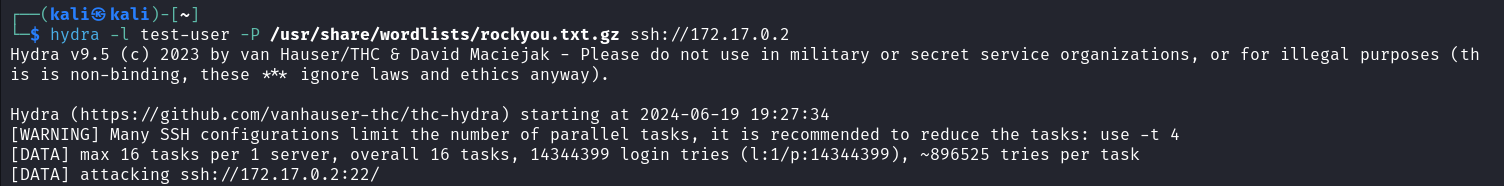
\includegraphics[width=1\linewidth]{imagenes/hydra-attack.png}
        \caption{Ataque por diccionario a servicio \gls{SSH} mediante Hydra}
        \label{fig:hydra-ssh}
\end{figure}

A continuación, se utilizó un \textit{scanner} de \texttt{Metasploit} para intentar enumerar usuarios de \gls{SSH} de las máquinas víctima. Para ello, se utilizaron los siguientes comandos:

\begin{center}
\begin{mdframed}
\scriptsize
    \begin{minted}{bash}
msfconsole # abrir una instancia de Metasploit
use auxiliary/scanner/ssh/ssh_enumusers # seleccionar script
set rhosts 172.17.0.2 # indicar la IP objetivo
set user_file /usr/share/wordlists/rockyou.gz # indicar el diccionario utilizado
run # ejecutar el ataque
    \end{minted}
\end{mdframed}
\end{center}

Finalmente, como se muestra en la Figura \ref{fig:metasploit-users}, se usa la técnica \textit{Malformed Packet}, que consiste en enviar paquetes formados incorrectamente a un servidor para probar forzar errores en el manejo de dichos paquetes y obtener información aparentemente oculta o inaccesible.

\begin{figure}[H]
    \centering
    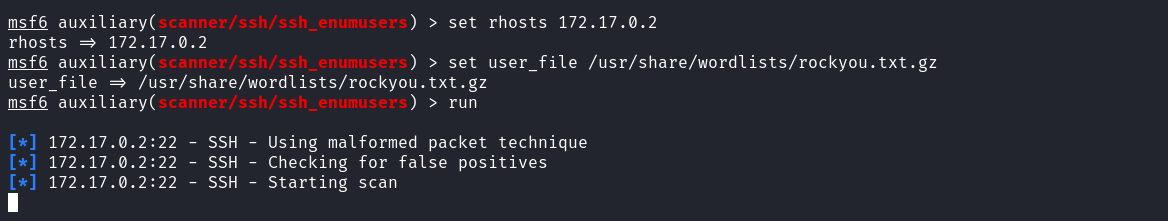
\includegraphics[width=1\linewidth]{imagenes/metasploit-attack.png}
    \caption{Ataque con Metasploit para enumeración de usuarios en un servidor \gls{SSH}}
    \label{fig:metasploit-users}
\end{figure}

\subsection{Dataset Sintético}

En el caso del conjunto de datos generado de manera sintética, se ha realizado por medio de la funcionalidad de análisis de datos utilizada por el LLM de OpenAI multimodal (\gls{GPT}4o). Para ello se ha hecho uso de técnicas de \textit{prompt engineering}, de modo que su estructura fuese equivalente a la del anterior \textit{dataset} ya preprocesado tal y como se especifica al final de la próxima sección \ref{fig:dataset-preprocesado}.

Este modelo es capaz de generar como salida un fichero de texto. Además, el \textit{notebook} que utiliza para generarlo puede ir readaptándose dinámicamente en base a las indicaciones que se van haciendo para ajustarlo al resultado deseado. Otra ventaja que presenta es la opción de adjuntar en el \textit{prompt} un fichero, de modo que si de añade un ejemplo del resultado esperado del conjunto de datos, como el generado anteriormente, el modelo razonará con más claridad como debe implementar las celdas de código. 

\begin{tcolorbox}[colframe=blue!25!white, colback=blue!10!white, title={\color{blue}\footnotesize \texttt{Prompt GPT4o - Generación Dataset Sintético}}]
\footnotesize
\textit{"Genera un archivo en formato \gls{CSV} que contenga 5000 registros, cada uno simulando un log de Linux orientado a la detección de vectores de ataque en sistemas de seguridad. Este dataset debe incluir una variedad ampliada de mensajes típicos encontrados en logs reales, adaptados para reflejar diversos tipos de actividades sospechosas y ataques, tales como intentos de acceso SSH, fallos de autenticación, alertas de kernel, y errores en aplicaciones y servicios de red. Cada log debe estar compuesto por las siguientes columnas, ajustándose al formato especificado en tu archivo de referencia: YYYY, MM, DD, hh, mm, Hostname, Service, User, IP, Port, Keyword, Interface, UID, Action, Protocol, Component, Severity, Type, Thread ID, Message.} \\
\end{tcolorbox}

\begin{tcolorbox}[colframe=blue!25!white, colback=blue!10!white, title={\color{blue}\footnotesize \texttt{Prompt GPT4o - Generación Dataset Sintético II}}]
\footnotesize
\textit{Incluye en los registros una mezcla de eventos legítimos y maliciosos, asegurando que los mensajes y tipos de errores sean coherentes con el protocolo y el servicio implicado (por ejemplo, mensajes ICMP relacionados con problemas de red y mensajes SSH relacionados con la autenticación). Asegúrate de que los datos sean variados y realistas para facilitar el análisis y la detección de patrones anómalos en aplicaciones de aprendizaje automático.} \\
\end{tcolorbox}

\begin{tcolorbox}[colframe=blue!25!white, colback=blue!10!white, title={\color{blue}\footnotesize \texttt{Prompt GPT4o - Generación Dataset Sintético III}}]
\footnotesize
\textit{El dataset debe ser guardado como} \verb|'06_Synthetic-logs-5k.csv'|\textit{, y cada entrada debe ser única para evitar redundancias y mejorar la calidad del mismo de cara a pruebas y entrenamiento de modelos."} \\

Por ejemplo:

\begin{tcolorbox}[colframe=white, colback=white, top=1mm, bottom=1mm, boxrule=0pt]
    \texttt{2024	05	05	09:38	f6194a3d2d4d	sshd[90]: test  172.17.0.1 	Invalid user test from 172.17.0.1 port 34132}
\end{tcolorbox}
\end{tcolorbox}

\vspace{2mm}

Además de los anteriores, fue necesario indicar 4 \textit{prompts} adicionales para ajustar más el formato del \textit{dataset} obtenido. Finalmente, se obtuvo el conjunto de datos que se muestra en la Figura \ref{fig:synthetic-dataset}, el cual incluye los veinte campos indicados, con una gran variedad de eventos y con una completitud significativa. 

\begin{figure}[H]
    \centering
    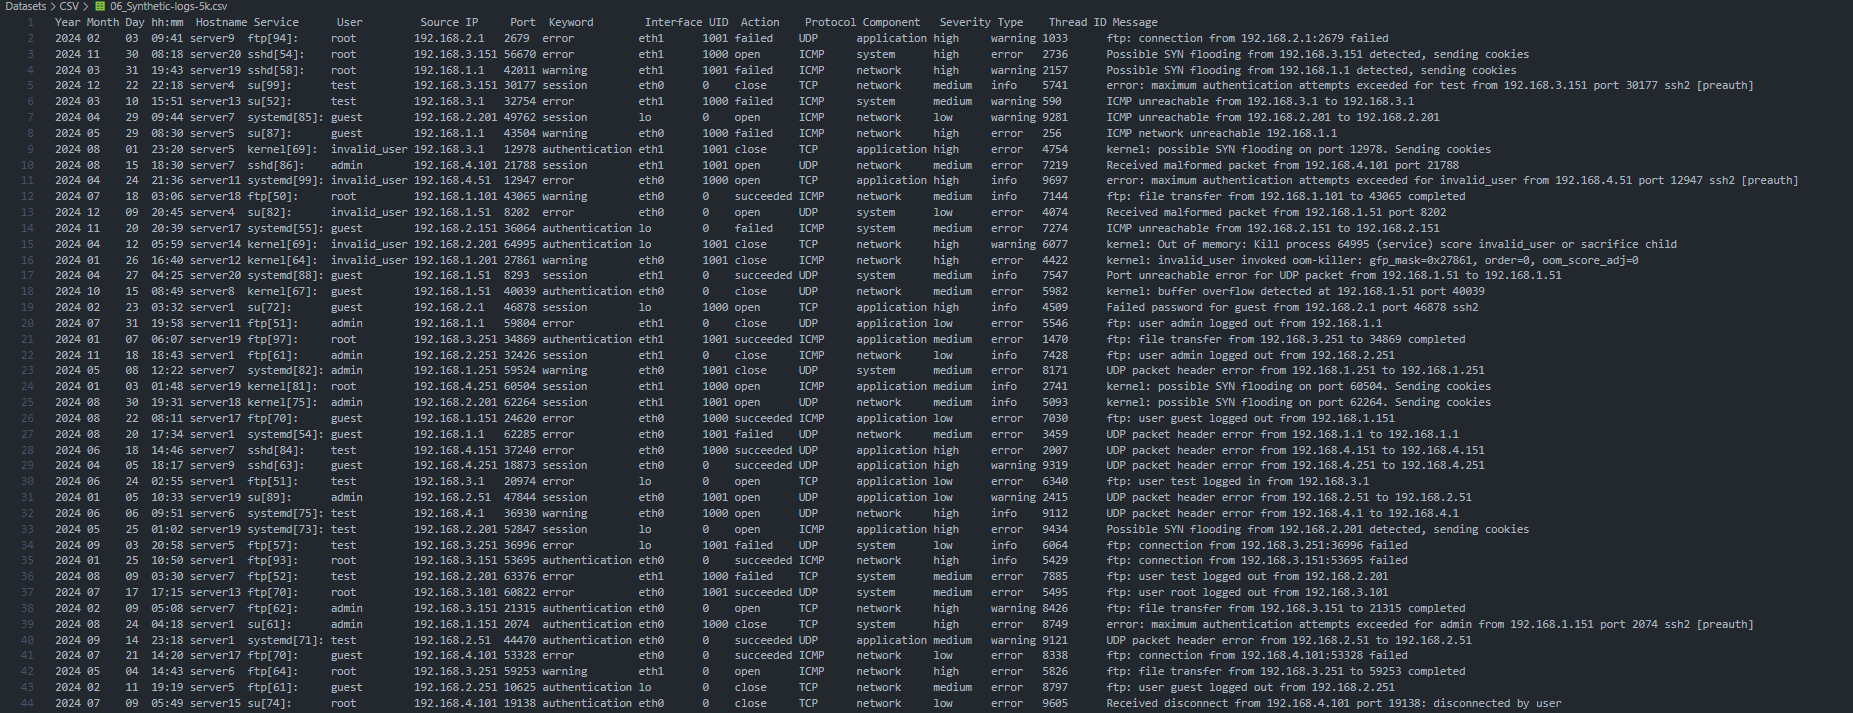
\includegraphics[width=1\linewidth]{imagenes/synthetic-dataset.png}
    \caption{Resultado del \textit{dataset} generado de forma sintética.}
    \label{fig:synthetic-dataset}
\end{figure}

Como se discute en el \textit{paper} de Krundyshev et. al \cite{inproceedings}, el uso de \textit{datasets} sintéticos en ciberseguridad actualmente es esencial para entrenar y evaluar modelos de detección de incidentes. Estos permiten simular una amplia gama de escenarios de ataque y actividades maliciosas que pueden no estar presentes en los datos reales debido a la rareza o sensibilidad de los incidentes. Además, ayudan a preservar la privacidad y la seguridad de los datos reales, mientras proporcionan un entorno controlado para experimentar y mejorar los modelos de detección. 


\newpage

% ********************************************************************

\section{Preparación de los \textit{dataset}s}


Una vez generado el \textit{dataset} original en formato \texttt{.log}, es necesario llevar a cabo un proceso de preprocesamiento de modo que pueda ser interpretado correctamente por los modelos de análisis de datos. Este proceso se tiene que realizar de manera equivalente para los otros \textit{datasets} que se han utilizado para hacer una comparativa y así enriquecer el análisis de posibles vectores de ataque. Se ha dividido en los siguientes pasos:

\begin{itemize}
    \item Limpieza del conjunto de datos: se eliminarán los eventos que se consideren residuales y no resulten útiles para el proceso de entrenamiento. Sin embargo, no se eliminarán todos los \textit{logs} que no estén relacionados con un ataque simulado, ya que la idea es poder generar agrupaciones de distintos \textit{logs} y ver cuáles de estas pertenecen a ataques, para que todo sea del modo más fidedigno posible a la realidad. 
    \item Preprocesamiento de los datos: el formato original de los \textit{logs} no es práctico para su análisis, por lo que será necesario transformarlo a un fichero \gls{CSV}, un formato más estandarizado para estas técnicas de \textit{clustering} y hacer técnicas de \textit{parsing} y normalización del texto.
    \item Extracción de características: en línea con el ítem anterior, será necesario extraer nuevos campos para facilitar el agrupamiento de \textit{logs} en base a características comunes.
\end{itemize}

A continuación se detalla cómo se han hecho cada uno de los pasos anteriores.

\vspace{-3mm}

\subsubsection*{Limpieza del conjunto de datos} % Dataset cleaning

En primer lugar, se suprimieron una gran cantidad de \textit{logs} redundantes y a su vez secuencialmente repetitivos para el problema a resolver, es decir, aquellos eventos generados en varias ocasiones que no aportaban al conjunto de datos. Este proceso se hizo manualmente examinando las aproximadamente nueve mil líneas de \textit{logs} y parseando a través de la técnica de \textit{search \& replace}. En la Figura \ref{fig:residual-logs} se muestra un ejemplo de \textit{logs} etiquetado como residual.

\vspace{-1mm}

\begin{figure}[H]
    \centering
    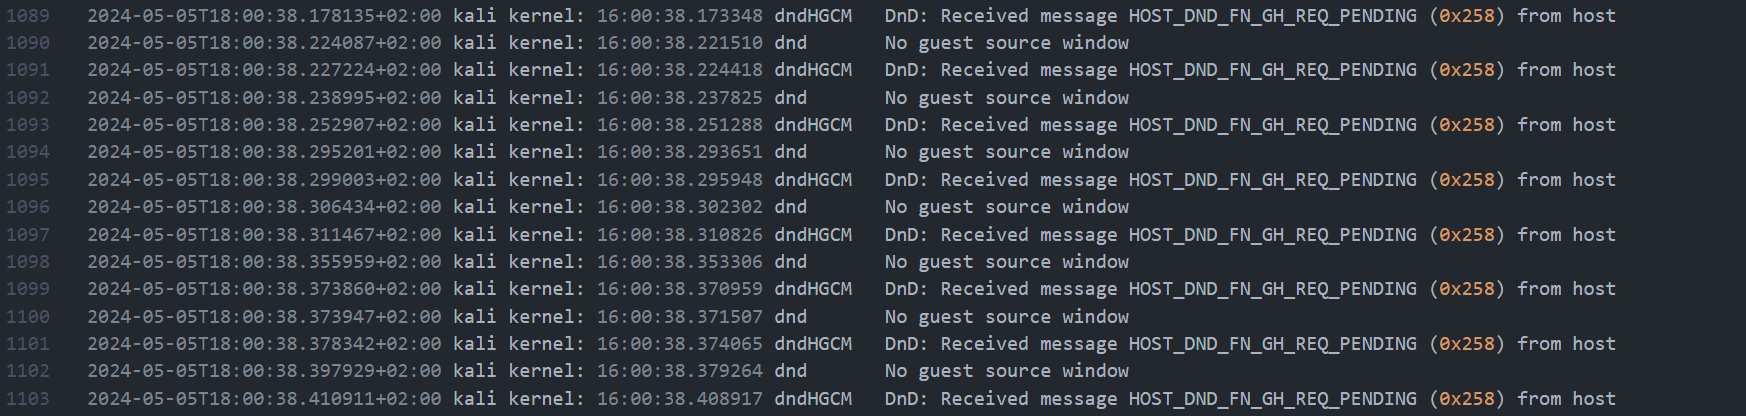
\includegraphics[width=1\linewidth]{imagenes/logs-residuales.png}
    \caption{Ejemplo de \textit{logs} residuales del conjunto de datos}
    \label{fig:residual-logs}
\end{figure}

\vspace{-5mm}

\begin{center}
\begin{mdframed}
\footnotesize
    \begin{minted}{bash}
No guest source window
DnD: Received message HOST_DND_FN_GH_REQ_PENDING (0x258) from host
    \end{minted}
\end{mdframed}
\end{center}

\vspace{-2mm}

Estos eventos están relacionados con un intento reiterado de realizar la operación de \gls{DnD} (\textit{drag \& drop}), pero que no se ha podido realizar debido a que no se ha encontrado la ventana de origen en el sistema invitado o \textit{guest}, un \textit{log} muy común en máquinas virtuales. También se han eliminado otros eventos relacionados con actividades de \textit{booting} de \gls{VM}s.

A través de este proceso, se consigue llevar a cabo un cierto balanceo de clases, lo cual es crucial para un buen rendimiento en el análisis de un \textit{dataset}. En el contexto de los conjuntos utilizados para este proyecto, el volumen de datos no es significativamente grande, sin embargo sería interesante usar algún algoritmo de balanceo \cite{garcia2021comparativa} en caso de enfrentarnos a conjuntos de datos mayores. Para ello se podrían utilizar algunos de los siguientes:

\begin{table}[H]
\centering
\footnotesize
\begin{tabularx}{\linewidth}{|>{\hsize=0.6\hsize}X|>{\hsize=1.4\hsize}X|}
\hline
\rowcolor{graylight}\texttt{Tipo} & \texttt{Descripción} \\
\hline
Sobremuestreo (\textbf{\textit{Oversampling}}) & Aumenta la cantidad de muestras en las clases menos representadas. El método más conocido es \gls{SMOTE} \cite{spositto2020smote}, donde se generan ejemplos sintéticos (no duplicados) mediante la interpolación entre ejemplos existentes de la clase minoritaria. \\
\hline
Submuestreo (\textbf{\textit{Undersampling}}) & Reduce la cantidad de muestras en las clases sobrerepresentadas. Este método puede llevar a una pérdida de información importante, pero es útil cuando hay un volumen muy alto de datos. \\
\hline
Combinación de sobremuestreo y submuestreo & Utiliza ambos métodos para equilibrar el conjunto de datos. Por ejemplo, se puede aplicar submuestreo a la clase mayoritaria y sobremuestreo a la clase minoritaria para lograr un balance. \\
\hline
Ensemble de modelos (\textbf{\textit{Ensemble methods}}) & Crea múltiples modelos (como árboles de decisión) en diferentes subconjuntos del conjunto de datos original, donde cada subconjunto refleja un balance de clases más equitativo. Técnicas como Balanced Random Forest o EasyEnsemble aplican esta idea. \\
\hline
Modificar pesos de clases (\textbf{\textit{Class weights modification}}) & Da más peso a la clase minoritaria durante el entrenamiento del modelo, lo cual puede influir en el algoritmo de aprendizaje para que preste más atención a la clase minoritaria. \\
\hline
\end{tabularx}
\caption{Técnicas de balanceo de clases para grandes conjuntos de datos}
\end{table}


\subsubsection*{Preprocesamiento de los datos}

Una vez los \textit{datasets} habían sido limpiados de \textit{logs} residuales, se pasó a la fase de preprocesamiento. Esta fase tuvo un primer enfoque mediante el cual los ficheros \textit{raw} se transformaron a un fichero \gls{JSON}.

El proceso fue muy similar para los conjuntos de datos utilizados. En el caso de los \textit{datasets} Linux\_2k \ref{Linux_2k} y el generado manualmente, se hizo uso de un mismo \textit{script}. Dicho código se adaptó levemente para poder utilizarse en los \textit{datasets} de \gls{BGL} (\ref{BGL}) y \gls{HDFS} (\ref{HDFS}). La principal diferencia entre estos fue el tratamiento del campo \textit{timestamp}, ya que los formatos eran ligeramente distintos, tal y como se explica en el capítulo cuarto (\ref{fig:linux-log-structure}).

\newpage

Para el primer paso, el \textit{script} realizaba un \textit{parsing} contenido para crear un diccionario con cuatro etiquetas por cada \textit{log}, de modo que se consiguiera la siguiente estructura:

\begin{center}
\begin{mdframed}
\footnotesize
    \begin{minted}{python}
{
    "timestamp": "2024-05-05T09:38:32+02:00",
    "hostname": "f6194a3d2d4d",
    "service": "sshd[90]:",
    "message": "pam_unix(sshd:auth): check pass; user unknown"
}
    \end{minted}
\end{mdframed}
\end{center}

Una vez todos los \textit{datasets} tenían este formato unificado, ya resultaba más fácil realizar el tratamiento de los campos para la extracción de características y generar nuevas columnas. 

\subsubsection*{Extracción de características}

Partiendo de los conjuntos de datos en formato \gls{JSON}, se continuó con el preprocesado. Se llevaron a cabo simultáneamente varios pasos \footnotemark para la extracción de características:


\begin{itemize}
    \item Normalización de los campos: principalmente, se normalizó el contenido del \textit{timestamp}, de modo que se mostrase con un formato equivalente. Este paso significó una leve pérdida de precisión en algunos de los datasets, que registraban también los segundos, microsegundos o bien la zona horaria asociada a la hora.
    \item Paso de \gls{JSON} a \gls{CSV}: mediante un \textit{notebook} de \textit{Jupyter} se llevó a cabo la transformación de los \textit{datasets} al formato matricial separado por comas. De esta manera, cada fila representaba un evento y cada columna una característica.
    \item Extracción de nuevos campos: a partir de los campos de \textit{timestamp} y \textit{message} se generaron nuevas columnas que mejorarían el potencial de estos para ser analizados y estudiados a continuación.
\end{itemize}

En este proceso se siguió una metodología equivalente al paso anterior, es decir, para los conjuntos de datos de \gls{HDFS} y \gls{BGL} se utilizaron \textit{notebooks} distintos al principal, que sí podía ser doblemente aprovechado por el \textit{dataset} generado manualmente y Linux\_2k, extraído de LogHub \cite{loghub2023}. Asimismo, los \textit{dataset} resultantes tienen un total de veinte columnas, siendo las primeras las relativas a los datos correspondientes al \textit{timestamp} separados en año, mes, día, hora, minutos y segundos, y la última columna el \textit{message} intacto. Las columnas intermedias son, además del servicio y el \textit{hostname}, aquellas que se han extraído de \textit{message}.

\footnotetext{Además de estos pasos, se hace uso de \gls{IDF}, pero esto será explicado más adelante en la próxima subsección (\ref{IDF})}


\begin{table}[H]
    \footnotesize
    \centering
    \begin{center}
        \begin{mdframed}
        \footnotesize
            \begin{minted}{python}
YYYY	MM	DD	hh:mm	Hostname     Service
2024	05	05	11:09	kali         sshd[90]: 
            \end{minted}
        \end{mdframed}
    \end{center}
    \begin{center}
        \begin{mdframed}
        \footnotesize
            \begin{minted}{python}
User    IP              Port	    Keyword	    Interface	
test    172.17.0.1      22              warning            eth0    
            \end{minted}
        \end{mdframed}
    \end{center}
    \begin{center}
        \begin{mdframed}
        \footnotesize
            \begin{minted}{python}
UID  	Action 	Protocol	Component	Severity
1000         Started        TCP             RAS              HIGH     
            \end{minted}
        \end{mdframed}
    \end{center}
    \begin{center}
        \begin{mdframed}
        \footnotesize
            \begin{minted}{python}
Type    Thread ID	 Message	    
INFO    357               Invalid user test from 172.17.0.1 port 22
            \end{minted}
        \end{mdframed}
    \end{center}
    \label{tab:my_label}
    \caption{Estructura del \textit{dataset} preprocesado}
\end{table}

En algunos casos, las columnas tienen más posibilidades de completarse en función del \textit{dataset} al que aplican, pero eso no significa que no puedan llegar a resultar de utilidad para la totalidad de los mismos. Por ese motivo y los mencionados anteriormente, he llegado a la conclusión de que todos los \textit{datasets} debían hacer uso de la misma estructura.

El \textit{parsing} se ha efectuado haciendo uso de los \gls{DF}s de la librería pandas, de modo que se aplicaban expresiones regulares sobre la columna de \textit{message} para identificar patrones que pudieran corresponderse con los nuevos campos extraídos. Por ejemplo, para llevar a cabo la extracción de una dirección \gls{IP} se implementó una función y luego esta era aplicada sobre el \textit{message} del \textit{dataframe}:

\begin{center}
\begin{mdframed}
\scriptsize
    \begin{minted}{python}
def extract_ip(message):
    match = re.search(r'\b(?:\d{1,3}\.\d{1,3}\.\d{1,3}\.\d{1,3})\b', message)
    return match.group(0) if match else None

df['IP'] = df['message'].apply(extract_ip)
    \end{minted}
\end{mdframed}
\end{center}

Otro ejemplo más sencillo es el de extracción del campo \textit{type}, donde se recorre el contenido de \textit{message} en busca de alguna de las palabras identificadas como los niveles de prioeridad (\ref{tab:syslog_priority}) o tipo de evento:

\begin{center}
\begin{mdframed}
\scriptsize
    \begin{minted}{python}
df['Type'] = df['message'].apply(lambda x:
re.findall(r'\b(INFO|FATAL|SEVERE|WARNING|ERROR|)\b', x, re.IGNORECASE)[0] if 
re.findall(r'\b(INFO|FATAL|SEVERE|WARNING|ERROR)\b', x, re.IGNORECASE) else None)

    \end{minted}
\end{mdframed}
\end{center}

Finalmente, se reorganiza el \textit{dataframe} añadiendo las nuevas columnas y utilizando una separación por tabulados. Dicha separación se podría llevar a cabo también con comas, de hecho es lo más común, sin embargo es visualmente más sencillo interpretar el contenido con columnas separadas con tabulaciones. Por tanto, las características extraídas de los \textit{datasets} de eventos son las siguientes: \\

\begin{itemize}
    \item \texttt{YYYY}: Año de registro del log. Indica el año de calendario en formato de cuatro dígitos. \\
    \item \texttt{MM}: Mes del registro en formato numérico. Representa el mes del evento del 01 (enero) al 12 (diciembre). \\
    \item \texttt{DD}: Día del mes del registro. Número del día del mes en que se registró el evento, de 01 hasta 31, dependiendo del mes. \\
    \item \texttt{hh}: Hora del registro en formato 24 horas, de 00 a 23. \\
    \item \texttt{mm}: Minuto del registro, de 00 a 59, detallando el minuto exacto de la hora en que ocurrió el evento. \\
    \item \texttt{Hostname}: Nombre del host donde se generó el registro, que identifica la máquina o servidor específico. \\
    \item \texttt{Service}: Nombre e identificador del servicio implicado en el registro, proporcionando detalles sobre el proceso o aplicación involucrada. \\
    \item \texttt{User}: Usuario asociado al evento del log. Detalla el nombre de usuario que ejecutó o desencadenó el evento, si aplica. \\
    \item \texttt{IP}: Dirección \gls{IP} asociada al registro. Especifica la dirección IP desde la cual se originó el evento, facilitando el rastreo de la actividad en la red. \\
    \item \texttt{Port}: Puerto de red relacionado con el evento. Indica el puerto de comunicación utilizado durante el incidente, si es relevante. \\
    \item \texttt{Keyword}: Palabras clave específicas identificadas en el mensaje. Ayuda a categorizar y buscar registros específicos basados en términos comunes. \\
    \item \texttt{Interface}: Interfaz de red implicada en el registro, proporcionando detalles sobre la interfaz física o virtual utilizada. \\
    \item \texttt{UID}: Identificador único del usuario asociado al registro, especialmente útil para correlacionar actividades en sistemas multiusuario. \\
    \item \texttt{Action}: Acción que describe el evento registrado, detallando la operación realizada, como iniciar, suspender, reanudar o finalizar una acción. \\
    \item \texttt{Protocol}: Protocolo de red relacionado con el registro, indicando el protocolo de comunicación utilizado (TCP, UDP, etc.), si aplica. \\
    \item \texttt{Component}: Componente del sistema implicado en el log, como un módulo específico del software o hardware involucrado. \\
    \item \texttt{Severity}: Nivel de severidad del evento, clasificado en términos de impacto o prioridad, como crítico, mayor, menor, o informativo. \\
    \item \texttt{Type}: Tipo de registro, basado en la naturaleza del evento, como error, advertencia, información, o depuración. \\
    \item \texttt{Thread ID}: Identificador del hilo de procesamiento asociado al evento, útil para el seguimiento de problemas en aplicaciones multihilo. \\
    \item \texttt{Message}: Mensaje detallado del registro, describiendo el evento, las acciones tomadas, y cualquier resultado relevante.
\end{itemize}

\begin{figure}[H]
    \centering
    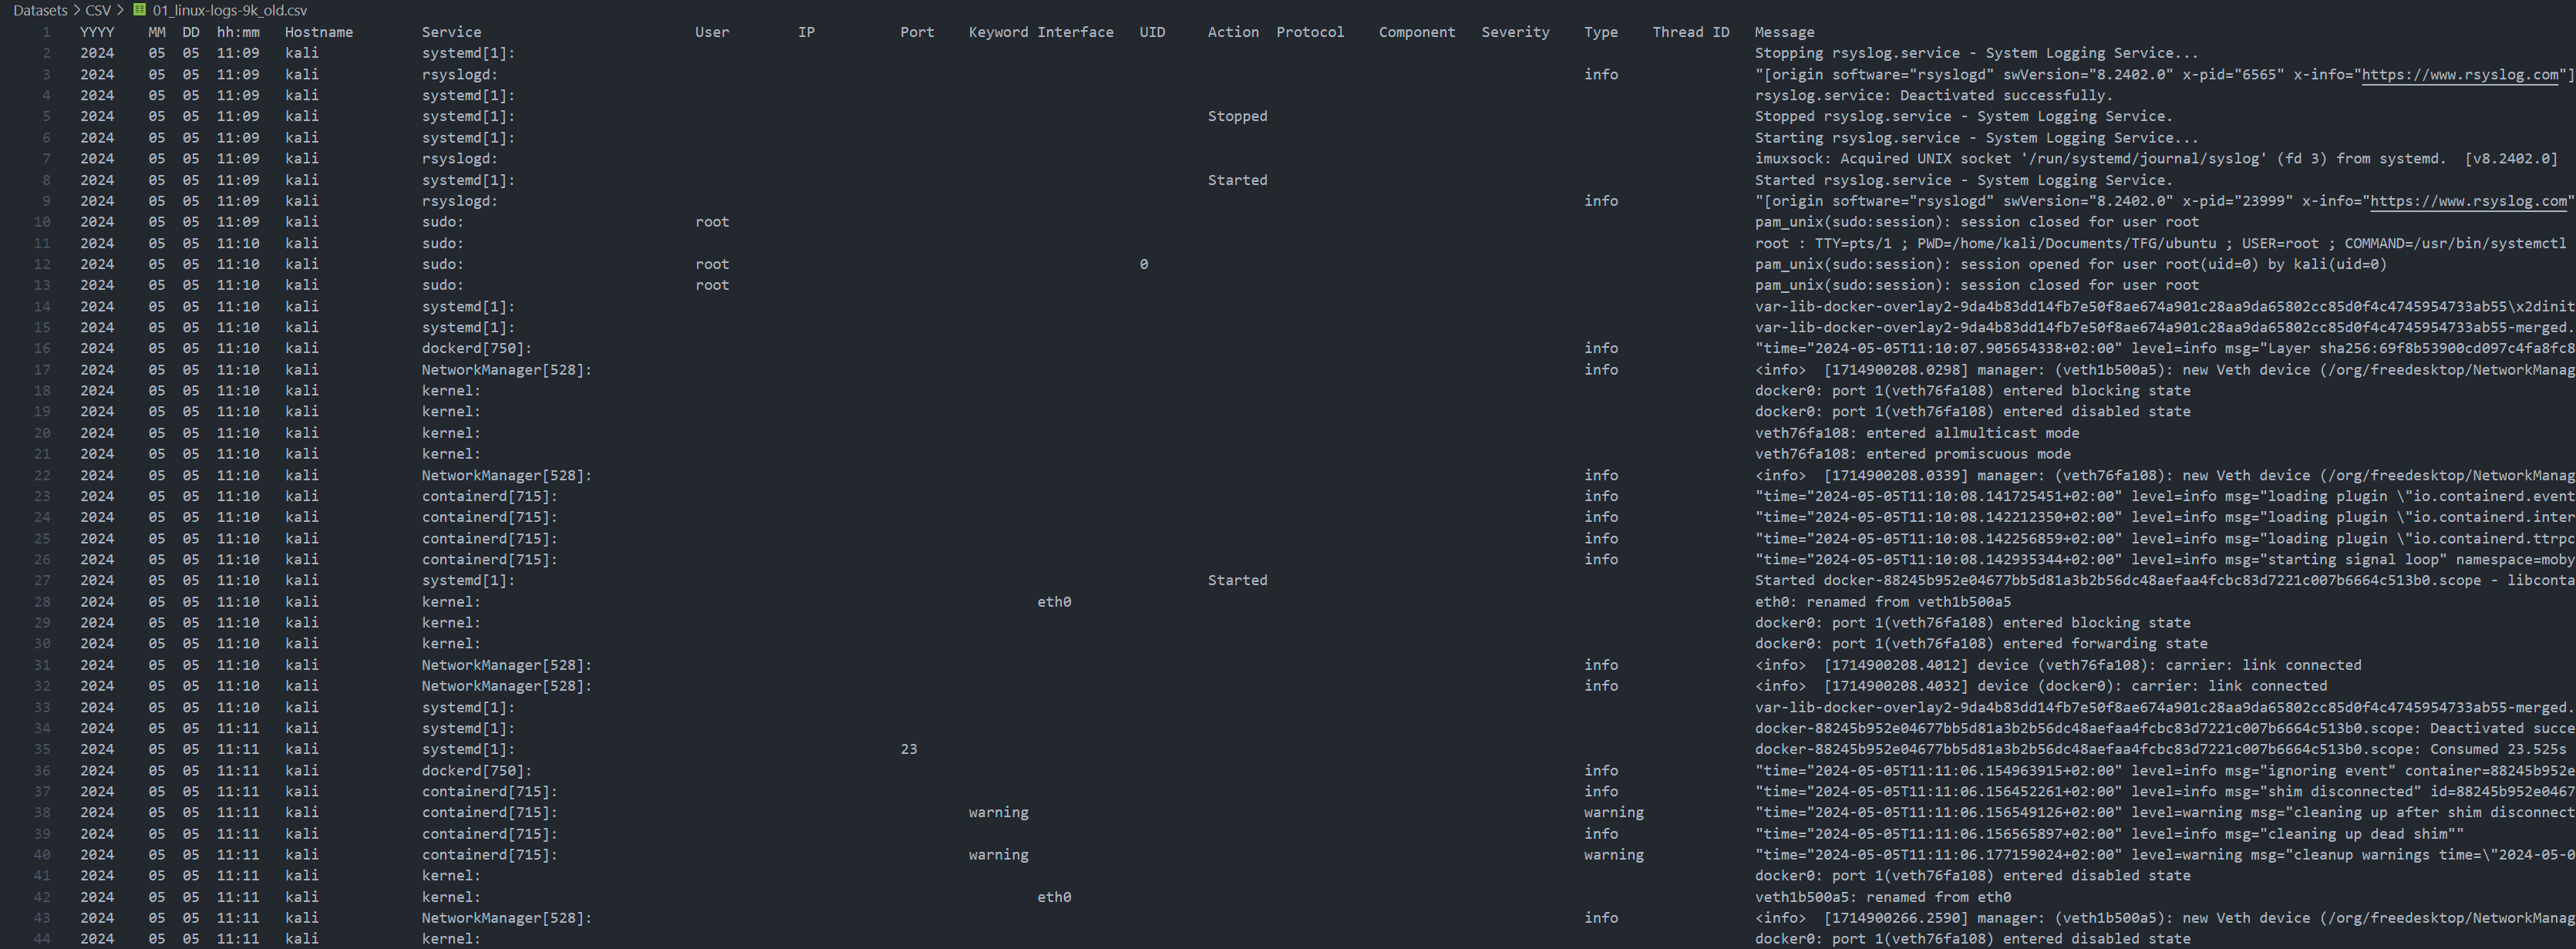
\includegraphics[width=1\linewidth]{imagenes/dataset-preprocesado.png}
    \caption{Estructura del \textit{dataset} tras fase de preprocesamiento}
    \label{fig:dataset-preprocesado}
\end{figure}

Tras este proceso de limpieza, preprocesamiento y extracción de características, los conjuntos de datos resultantes que serán usados para realizar el \textit{clustering} tienen las siguientes características:

\begin{table}[H]
\centering
\footnotesize
\begin{tabularx}{\textwidth}{|X|r|}
\hline
\rowcolor{graylight}\texttt{Nombre} & \texttt{Nº de eventos} \\ 
\hline
01\_linux-logs-9k.csv & 8890 \\ 
\hline
02\_linux-logs-2k.csv & 1546 \\ 
\hline
03\_HDFS-logs-20k.csv & 20000 \\ 
\hline
04\_BGL-logs-20k.csv & 20000 \\ 
\hline
05\_Synthetic-logs-5k.csv & 5000 \\
\hline
06\_auth-logs-20k.csv & 20000 \\
\hline
\end{tabularx}
\caption{Listado de conjuntos de datos preprocesados}
\label{tab:conjuntos-datos}
\end{table}

De los conjuntos de datos presentados en la Tabla \ref{tab:conjuntos-datos}, tres de ellos (03\_HDFS-logs-20k.csv, 04\_BGL-logs-20k.csv y 06\_auth-logs-20k.csv) son fragmentos de otros \textit{datasets} de mayor tamaño, que se han limitado a 20000 eventos. La decisión de no tomar los originales se ha sustentado en las limitaciones de cómputo disponibles para este Trabajo. Sin embargo, podría realizarse el mismo proceso utilizando sus versiones originales en caso de disponer de los recursos necesarios.

% ********************************************************************

\newpage

\section{Implementación del modelo}

Seguidamente, se llevó a cabo la implementación de distintos algoritmos de \textit{clustering} para clasificar los conjuntos de datos generados, y en base a los resultados obtenidos extraer potenciales vectores de ataque. A continuación se muestran las técnicas de vectorización de texto, reducción de dimensionalidad y extracción de características utilizadas, así como los pasos seguidos para implementar los algoritmos de agrupación.

\subsection{Técnicas utilizadas}

Se ha hecho uso de distintas técnicas que mejorasen la creación de agrupaciones de eventos para que estas fueran procesadas de forma más precisa, y otras técnicas para minimizar la cantidad de dimensiones y simplificar los datos sin perder la representatividad.

\subsubsection*{Técnicas de Vectorización de Texto}

La vectorización de texto se utiliza para transformar cada uno de los eventos de \textit{logs} en representaciones numéricas, de modo que estos puedan ser procesados por algoritmos de \gls{ML}. Para ello, se han utilizado las siguientes herramientas: \\

\textbf{\gls{TF}-\gls{IDF}}: (\textit{Term Frequency-Inverse Document Frequency}): convierte los \textit{logs} en una matriz de características \gls{TF}-\gls{IDF}. Como indica su acrónimo, puede desglosarse en dos partes con distinta funcionalidad:
\begin{itemize}
    \item \textbf{\gls{TF}} (\textit{Term Frequency}): en primer lugar, este mide la frecuencia de cada una de las palabras existentes en una línea y posteriormente las vectoriza, convirtiéndolas en un conjunto de números que representan la frecuencia de cada palabra en dicho documento \footnotemark. \\
    \item \textbf{\gls{IDF}} (\textit{Inverse Document Frequency}) \label{IDF}: en segundo lugar, se reduce la escala de las palabras que aparecen con mayor frecuencia en el conjunto de documentos o \textit{corpus}, y que por consiguiente son más discriminatorias con respecto a las demás palabras. Esto ayuda a resaltar aquellas palabras que son más únicas para cada \textit{dataset} de eventos de Linux. \\
\end{itemize}

\footnotetext{Cuando se habla de documentos en este contexto, nos referimos a una línea o conjunto de líneas del \textit{dataset}.}

A efectos matemáticos, según Ho Chung et. al \cite{tf-idf} se interpreta como el producto de las dos medidas, \gls{TF} e \gls{IDF}. Su valor puede calcularse de varias formas:

Por un lado, \textbf{\gls{TF}}, representado como tf(t, d), se suele usar la \textit{frecuencia bruta} del término t en el \textit{dataset} d, es decir, el nº de veces que una palabra o término t aparece en d. Denotando la frecuencia bruta de t por f(t,d), la función tf será tf(t, d) = f(t,d). También se pueden utilizar otras alternativas como las frecuencias booleanas, escalada logarítmicamente o la normalizada. 

\newpage

Esta última se calcula por el cociente de la frecuencia bruta entre la frecuencia máxima de alguna palabra (t) en el documento:

\begin{equation}
    \text{tf}(t, d) = \frac{f(t, d)}{\max\{f(t', d) : t' \in d\}}
\end{equation}

Por otro lado, \textbf{\gls{IDF}} mide si la palabra es común o no en el conjunto de \textit{corpus}. Se obtiene por medio del cociente del nº total de \textit{datasets} entre el número de \textit{datasets} que contienen la palabra, y se toma el logaritmo de dicho cociente:

\begin{equation}
    \text{idf}(t, D) = \log \left( \frac{|D|}{|\{d \in D : t \in d\}|} \right)
\end{equation}

donde:

\begin{itemize}
    \item $|D|$: cardinalidad de D, o número de \textit{datasets} en el conjunto. \\
    \item $|\{d \in D : t \in d\}|$: número de \textit{datasets} donde aparece la palabra o término t. Si no está en la colección se producirá una división-por-cero. Por lo tanto, es común ajustar esta fórmula a $1 + |\{d \in D : t \in d\}|$.
\end{itemize}

Por último, en cuanto a la base de la función \textit{log} no es relevante con respecto al resultado final obtenido. Por tanto, \gls{TF}-\gls{IDF} se calcula de la siguiente forma:

\begin{equation}
    \text{tfidf}(t, d, D) = \text{tf}(t, d) \times \text{idf}(t, D)
\end{equation}

La combinación de estos permite por tanto la vectorización de los \textit{logs} y al mismo tiempo la extracción de sus características. De cara a su uso en el \textit{notebook}, se han importado de la librería Sci-kit Learn (\ref{scikit}):

\begin{center}
    \begin{mdframed}
    \scriptsize
            \begin{minted}{javascript}
from sklearn.feature_extraction.text import TfidfVectorizer
            \end{minted}
    \end{mdframed}
\end{center}

La segunda técnica utilizada ha sido \textbf{Count-Vectorizer} \cite{scikit_count_vectorizer}. Esta herramienta se utiliza para transformar un \textit{dataset} de texto en una matriz numérica de recuentos de palabras.

A diferencia de \gls{TF}-\gls{IDF}, Count-Vectorizer simplemente cuenta la frecuencia de aparición de cada término en el documento, sin considerar la frecuencia inversa de los documentos. Esta es útil cuando se desea obtener una representación simple y directa de la frecuencia de los términos.

Su proceso puede describirse de la siguiente manera:

\begin{enumerate}
    \item Primero, se construye un vocabulario con todos los términos únicos presentes en el \textit{corpus}.
    \item Luego, se cuenta la frecuencia de aparición de cada término en cada línea, creando así una matriz en la que las filas representan líneas y las columnas representan los términos del vocabulario.
    \item Cada entrada en la matriz corresponde al número de veces que un término aparece en una línea específica.
\end{enumerate}

Este método es más sencillo y rápido de computar en comparación con \gls{TF}-\gls{IDF}, pero no proporciona la misma capacidad para diferenciar términos comunes y poco comunes en el conjunto de documentos. En el \textit{notebook}, se ha importado y utilizado de la librería Sci-kit Learn (\ref{scikit}) de la siguiente manera:

\begin{center}
    \begin{mdframed}
    \scriptsize
            \begin{minted}{javascript}
from sklearn.feature_extraction.text import CountVectorizer
            \end{minted}
    \end{mdframed}
\end{center}

De cara a futuras mejoras sería interesante utilizar otras alternativas como Word2Vec que aprende asociaciones de palabras a partir de grandes cantidades de datos en texto plano, y \gls{BERT}, o su versión adaptada a detección de anomalías de seguridad como \gls{BERT}-log \cite{guo2021logbert}.

\vspace{-2mm}

\subsubsection*{Técnicas de Reducción de Dimensionalidad}

La reducción de dimensionalidad en los \textit{corpus} de \textit{logs} ha implicado transformar datos complejos en una representación más simple y manejable, sin perder mucha información importante. Para lograr esto, se han utilizado tres técnicas distintas.

En primer lugar, \textbf{\gls{PCA}} (\textit{Principal Component Analysis}) \cite{Jolliffe2016PCA} transforma los datos a un nuevo sistema de coordenadas donde las mayores varianzas de los datos se proyectan en las primeras coordenadas. Esto permite reducir la dimensionalidad del \textit{corpus} de \textit{logs} manteniendo la mayor cantidad de varianza posible. Esta técnica es escalable a conjuntos de datos de un mayor tamaño, pero puede no capturar adecuadamente las complejas relaciones no lineales presentes en los \textit{logs} de eventos de seguridad, lo que puede afectar la precisión en la detección de patrones de ataque. 

Para utilizarla en el \textit{notebook}, se realiza el siguiente \textit{import}:

\begin{center}
    \begin{mdframed}
    \scriptsize
            \begin{minted}{javascript}
from sklearn.decomposition import PCA
            \end{minted}
    \end{mdframed}
\end{center}

En segundo lugar, \textbf{\gls{t-SNE}} (\textit{t-distributed Stochastic Neighbor Embedding}) \cite{Maaten2008tSNE}, convierte similitudes entre datos en alta dimensión en probabilidades conjuntas y minimiza la divergencia de Kullback-Leibler entre estas probabilidades en el espacio de baja dimensión. Esta es particularmente efectiva para la agrupación de eventos de \textit{logs}, ya que puede capturar relaciones no lineales y resaltar estructuras de \textit{clusters} que son críticas para la identificación de vectores de ataque. Sin embargo, \gls{t-SNE} puede ser computacionalmente costoso y no escalar bien con conjuntos de datos muy grandes, lo que podría limitar su aplicabilidad en escenarios con grandes volúmenes de datos de \textit{logs}. Se importa de la siguiente forma:

\begin{center}
    \begin{mdframed}
    \scriptsize
            \begin{minted}{javascript}
from sklearn.manifold import TSNE
            \end{minted}
    \end{mdframed}
\end{center}

Por último, \textbf{\gls{UMAP}} (\textit{Uniform Manifold Approximation and Projection}) \cite{McInnes2018UMAP} está basada en la teoría de grafos y la topología algebraica, por lo que preserva tanto la estructura local como global de los datos. \gls{UMAP} puede manejar grandes conjuntos de datos de manera eficiente y mantener la integridad de las relaciones tanto locales como globales. Esto facilita la detección de patrones complejos y anómalos en los \textit{logs} con relativa rapidez pero, en consecuencia, solamente es útil para un número de vecinos pequeño. Para hacer uso de esta, primero es necesario instalar la dependencia de \verb|umap-learn| y luego hacer el \textit{import}:

\begin{center}
    \begin{mdframed}
    \scriptsize
            \begin{minted}{javascript}
!pip install umap-learn
import umap.umap_ as umap
            \end{minted}
    \end{mdframed}
\end{center}

A través de todas las técnicas que han sido mencionadas, se tratará de mejorar el tratamiento de los \textit{dataset} y así obtener unos mejores resultados. Algunas de ellas serán combinadas y se analizará su rendimiento por medio de comparativas.

\subsection{Desarrollo del \textit{clustering}}

Una vez aplicadas las técnicas mencionadas anteriormente tanto para la vectorización de texto como para la reducción de la dimensionalidad, se ha llevado a cabo la implementación de los algoritmos de \textit{clustering} escogidos en el capítulo anterior. En el caso del \textit{clustering} jerárquico, se han utilizado tanto el algoritmo \gls{HC}, como la variante aglometariva: \gls{AHC}. A continuación se detalla el procedimiento seguido para cada uno de ellos.

Con el propósito de ir validando e ir haciendo un primer análisis sobre los resultados obtenidos, se ha ido imprimiendo un conjunto de gráficas, correspondientes a cada una de las combinaciones entre técnicas y algoritmos de \textit{clustering}, de modo que se estimara visualmente qué combinación respondía mejor frente a este tipo de de \textit{corpus}.


En esta sección, se mostrará el proceso para el tratamiento del conjunto de datos generado manualmente, es decir: \textit{01\_linux-logs-9k.csv}. En el caso de los demás \textit{datasets} se ha seguido estrictamente el mismo procedimiento. Por lo que en el próximo capítulo se analizarán y compararán los resultados obtenidos.

\subsubsection*{Implementación de K-means}

En primer lugar, para K-means se ha realizado la estimación del número óptimo de \textit{clusters} asociado al parámetro \textit{k} por medio del Algoritmo del Codo\footnotemark, mencionado en el capítulo cuarto \ref{fig:metodo-codo}. En la Figura \ref{fig:codo-manual} se muestran resultados obtenidos para el \textit{dataset} \textit{01\_linux-logs-9k.csv}.

Como se observa, pueden diferenciarse ligeramente tres codos. El primero de ellos en torno a \textit{k=5}, el segundo alrededor de \textit{k=10} y el último próximo a \textit{k=16}. Con el fin de verificar cual de estos valores es el más óptimo, se ha utilizado \textit{Silhouette Score} en el rango [2,31].

\newpage

\begin{figure}[H]
    \centering
    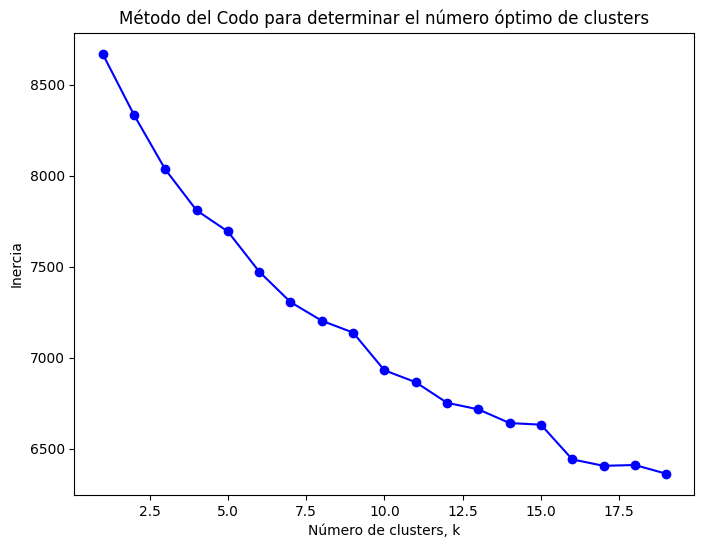
\includegraphics[width=0.95\linewidth]{imagenes/algoritmo-codo.png}
    \caption{Aplicación del Algoritmo del Codo sobre \textit{dataset} generado manualmente}
    \label{fig:codo-manual}
\end{figure}

\footnotetext{En la Figura \ref{fig:codo-manual} el eje \textit{y} está sociado a la Inercia, que es la suma de las distancias cuadradas de cada punto al centro de su \textit{cluster} más cercano.}


\begin{figure}[H]
    \centering
    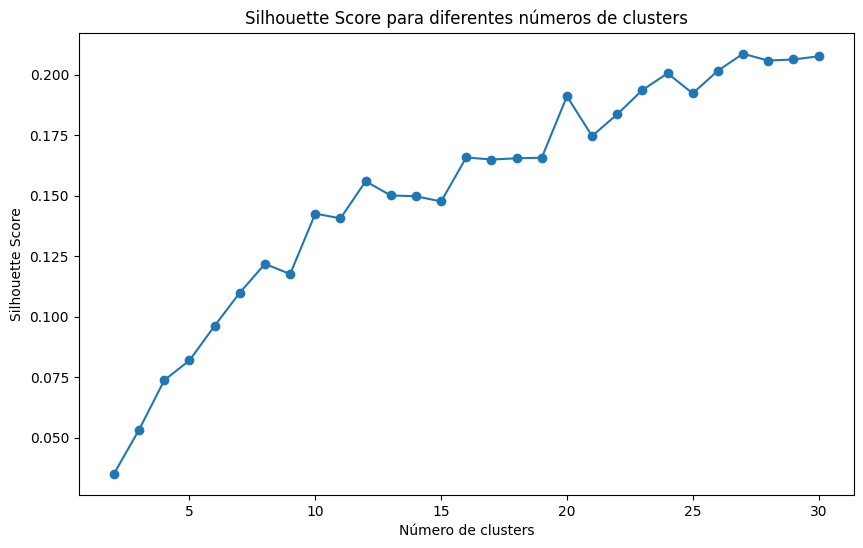
\includegraphics[width=0.95\linewidth]{imagenes/kmeans-silhouette.png}
    \caption{Cálculo del valor \textit{k} óptimo mediante Silhouette Score}
    \label{fig:kmeans-silhouette-optimo}
\end{figure}

\newpage

En base a los resultados visibles en la Figura \ref{fig:kmeans-silhouette-optimo}, no se observa ningún pico especialmente significativo salvo uno cercano a \textit{k=10}. Esto se debe a la heterogeneidad de los \textit{logs}, incluso aquellos asociados a ataques de fuerza bruta. Si el rango utilizado para aplicar \textit{Silhouette Score} aumentara, se ampliaría la cantidad de \textit{clusters}, pero lo más conveniente es seleccionar un número realista, por tanto se fijará \textit{k=10}.

Ahora se debe de llevar a cabo la inicialización del algoritmo utilizando 10 \textit{clusters} y un valor fijo para la semilla (en este caso 42), que será utilizada posteriormente para poder comparar todos los resultados obtenidos. Seguidamente se aplicará el algoritmo al \textit{dataset X}, de modo que se guarden todas las etiqutetas de \textit{cluster} asignadas a cada punto en \textit{kmeans\_labels}. 

\begin{center}
    \begin{mdframed}
    \footnotesize
            \begin{minted}{rust}
kmeans = KMeans(n_clusters=10, random_state=42)
kmeans_labels = kmeans.fit_predict(X)
            \end{minted}
    \end{mdframed}
\end{center}


Por último se añadirá al \gls{DF} una columna adicional que identificará la etiqueta de \textit{cluster} que le corresponda y se extraerán las características más representativas de cada uno de estos diez \textit{clusters}, de modo que pueda visualizarse posteriormente.


\begin{center}
    \begin{mdframed}
    \footnotesize
            \begin{minted}{rust}
data['kmeans_cluster'] = kmeans_labels
kmeans_cluster_terms = np.array([extract_cluster_terms(kmeans_labels, 
features, X.toarray())[i] for i in range(10)])
            \end{minted}
    \end{mdframed}
\end{center}

\subsubsection*{Implementación de \gls{DBSCAN}}

Para el caso de \gls{DBSCAN}, no se especifica directamente el número de \textit{clusters}, sino que se calcula en base a los parámetros \textit{eps} y \textit{min\_samples}. Tras realizar pruebas prácticas para ver qué valores respondían mejor, se han establecido los siguientes:

\[eps = 0.5, min\_samples = 5\]

\begin{center}
    \begin{mdframed}
    \footnotesize
            \begin{minted}{rust}
dbscan = DBSCAN(eps=0.5, min_samples=5)
dbscan_labels = dbscan.fit_predict(X)
            \end{minted}
    \end{mdframed}
\end{center}

Tras inicializar el algoritmo con los valores especificados, y a continuación aplicarlo al \textit{dataset}, se procede a añadir al \textit{dataframe} la nueva eiquetas y extraer las características.

\begin{center}
    \begin{mdframed}
    \footnotesize
            \begin{minted}{rust}
data['dbscan_cluster'] = dbscan_labels
dbscan_cluster_terms = extract_cluster_terms(dbscan_labels, features, 
X.toarray())
            \end{minted}
    \end{mdframed}
\end{center}

\newpage

\subsubsection*{Implementación de \gls{AHC} y \gls{HC}}

Para los algoritmos de \textit{clustering} jerárquico y aglomerativo, se ha optado por emplear el método de enlace \textit{ward}, que minimiza la suma de diferencias cuadradas dentro de todos los \textit{clusters}. Este método es menos susceptible a ruido y \textit{outliers} en comparación con otros métodos de enlace como el completo o el simple. Este utiliza la siguiente fórmula para calcular la distancia entre dos \textit{clusters} \(A\) y \(B\):

\[
    D(A,B) = \sqrt{\frac{|A| \times |B|}{|A| + |B|} \times ||\text{centroide}_A - \text{centroide}_B||^2}
\]

Después de calcular las distancias utilizando el método de enlace \textit{ward}, el siguiente paso es aplicar la función \textit{linkage} para construir la jerarquía de agrupaciones y luego usar \textit{fcluster} para formar los \textit{clusters}. De esta forma, será posible visualizar los dendogramas generados para poder hacer el análisis.

\begin{center}
    \begin{mdframed}
    \footnotesize
            \begin{minted}{rust}
linked = linkage(X.toarray(), method='ward') 
hierarchical_labels = fcluster(linked, 10, criterion='maxclust')
            \end{minted}
    \end{mdframed}
\end{center}

Una vez etiquetados los \textit{clusters}, se deben asignar estas etiquetas a los datos originales, de modo que puedan identificarse características comunes dentro de cada \textit{cluster}.

\begin{center}
    \begin{mdframed}
    \footnotesize
            \begin{minted}{rust}
data['hierarchical_cluster'] = hierarchical_labels
hierarchical_cluster_terms = extract_cluster_terms(hierarchical_labels, 
features, X.toarray())
            \end{minted}
    \end{mdframed}
\end{center}

En el caso del \textit{clustering} aglomerativo es similar al jerárquico pero con un enfoque más directo en la combinación progresiva de \textit{clusters} hasta alcanzar el número deseado de agrupaciones. Este método tenderá a dar mejores resultados con los \textit{datasets} con mayor volumen de datos, como se demostrará en el próximo capítulo.

\begin{center}
    \begin{mdframed}
    \footnotesize
            \begin{minted}{rust}
agglomerative_clustering = AgglomerativeClustering(n_clusters=9)
agglomerative_labels = agglomerative_clustering.fit_predict(X.toarray())
            \end{minted}
    \end{mdframed}
\end{center}

Finalmente, los resultados del \textit{clustering} aglomerativo se asignan a los datos, y se extraen términos representativos para cada \textit{cluster}.

\begin{center}
    \begin{mdframed}
    \footnotesize
            \begin{minted}{rust}
data['agglomerative_cluster'] = agglomerative_labels
agglomerative_cluster_terms = extract_cluster_terms(agglomerative_labels, 
features, X.toarray())
            \end{minted}
    \end{mdframed}
\end{center}

% ********************************************************************

\newpage

\section{Selección de métricas de evaluación}

El análisis del \textit{clustering} en el contexto de la detección de patrones de ataque en \textit{logs} requiere unas métricas específicas que reflejen la calidad de la agrupación más que la precisión de clasificación. Por este motivo, métricas comunes en otros contextos de aprendizaje supervisado como RECALL, PRECISION, o F1 Score no son aplicables aquí, ya que presuponen la existencia de etiquetas verdaderas previas, lo cual no se alinea con la naturaleza no supervisada del \textit{clustering} \cite{Rousseeuw1987}.

\subsubsection*{Silhouette Score}

El coeficiente de silueta mide cuán bien un objeto está emparejado a su propio \textit{cluster} comparado con otros clusters. Este coeficiente varía de -1 a 1, donde valores cercanos a 1 indican una asignación adecuada del objeto a su \textit{cluster}. La fórmula del coeficiente de silueta es:

\begin{equation}
    s = \frac{b - a}{\max(a, b)}
\end{equation}

donde \(a\) es la distancia media dentro del \textit{cluster} y \(b\) es la menor distancia media a cualquier otro cluster del que el objeto no es miembro.

Esta métrica viene implementada en \texttt{Python} a través dela librería \texttt{scikit-learn} (\ref{scikit}). Para ello, se utiliza el siguiente bloque de código:

\begin{center}
    \begin{mdframed}
    \scriptsize
            \begin{minted}{javascript}
from sklearn.metrics import silhouette_score
            \end{minted}
    \end{mdframed}
\end{center}

\subsubsection*{Índice de Davies-Bouldin}

El índice de Davies-Bouldin \cite{DaviesBouldin1979} es una métrica que evalúa la separación entre \textit{clusters}. Valores más bajos de este índice indican que los \textit{clusters} están bien separados y son compactos. La fórmula para calcular el índice de Davies-Bouldin \cite{petrovic2006comparison} es la siguiente:

\begin{equation}
    DB = \frac{1}{n} \sum_{i=1}^{n} \max_{j \neq i} \left( \frac{\sigma_i + \sigma_j}{d(c_i, c_j)} \right)
\end{equation}

donde \(\sigma\) es la dispersión dentro del \textit{cluster} y \(d(c_i, c_j)\) es la distancia entre los centroides de los clusters \(i\) y \(j\).

\vspace{2mm}

Al igual que la anterior, esta métrica viene implementada en \texttt{Python} por medio de \texttt{scikit-learn}. Puede importarse con:

\begin{center}
    \begin{mdframed}
    \scriptsize
            \begin{minted}{javascript}
from sklearn.metrics import davies_bouldin_score
            \end{minted}
    \end{mdframed}
\end{center}

\newpage

\subsubsection*{Índice de Calinski-Harabasz}

Por último, el índice de Calinski-Harabasz \cite{CalinskiHarabasz1974} compara la dispersión entre los \textit{clusters} con la dispersión existente dentro de los \textit{clusters}. Valores más altos indican una mejor definición de los \textit{clusters}. La fórmula para el índice de Calinski-Harabasz es:

\begin{equation}
    CH = \frac{SSB / (k - 1)}{SSW / (n - k)}
\end{equation}

donde \(SSB\) es la suma de cuadrados entre los \textit{clusters}, \(SSW\) es la suma de cuadrados dentro de los \textit{clusters}, \(k\) es el número de \textit{clusters}, y \(n\) es el número de puntos.

Para importar esta métrica se usa una vez más la implementación proporcionada por \texttt{scikit-learn}:

\begin{center}
    \begin{mdframed}
    \scriptsize
            \begin{minted}{javascript}
from sklearn.metrics import calinski_harabasz_score
            \end{minted}
    \end{mdframed}
\end{center}

Para calcular en el \textit{notebook} las distintas métricas utilizadas, se he hecho uso del siguiente fragmento de código:

\begin{center}
    \begin{mdframed}
    \scriptsize
            \begin{minted}{javascript}
metrics = {
    'Método de Clustering': ['K-Means', 'DBSCAN', 'Clustering Jerárquico', 
    'Clustering Jerárquico Aglomerativo'],
    'Silhouette Score': [
        silhouette_score(X, kmeans_labels),
        silhouette_score(X, dbscan_labels) if len(set(dbscan_labels)) > 1 
        else "No aplicable",
        silhouette_score(X, hierarchical_labels),
        silhouette_score(X, agglomerative_labels)
    ],
    'Índice Davies-Bouldin': [
        davies_bouldin_score(X.toarray(), kmeans_labels),
        davies_bouldin_score(X.toarray(), dbscan_labels) 
        if len(set(dbscan_labels)) > 1 else "No aplicable",
        davies_bouldin_score(X.toarray(), hierarchical_labels),
        davies_bouldin_score(X.toarray(), agglomerative_labels)
    ],
    'Índice Calinski-Harabasz': [
        calinski_harabasz_score(X.toarray(), kmeans_labels),
        calinski_harabasz_score(X.toarray(), dbscan_labels) 
        if len(set(dbscan_labels)) > 1 else "No aplicable",
        calinski_harabasz_score(X.toarray(), hierarchical_labels),
        calinski_harabasz_score(X.toarray(), agglomerative_labels)
    ]
}
            \end{minted}
    \end{mdframed}
\end{center}

\newpage


Por tanto, los valores que pueden tomar los resultados utilizando las métricas mencionadas pueden corresponden con los de la Tabla \ref{tab:intervalos_metricas}.

\begin{table}[H]
\centering
\footnotesize
\begin{tabularx}{\textwidth}{|X|r|r|}
\hline
\rowcolor{graylight}\texttt{Métrica} & \texttt{Mínimo} & \texttt{Máximo} \\ 
\hline
Coeficiente de Silueta & -1 & 1 \\ 
\hline
Índice de Davies-Bouldin & 0 & $\infty$ \\
\hline
Índice de Calinski-Harabasz & 0 & $\infty$ \\
\hline
\end{tabularx}
\caption{Intervalos de oscilación para las métricas de evaluación del \textit{clustering}}
\label{tab:intervalos_metricas}
\end{table}

\subsubsection*{Extracción de términos principales}

Además de llevar a cabo el análisis del \textit{clustering} por medio de las tres métricas mencionadas anteriormente, se han implementado varias funciones que permitan extraer las palabras clave asoaciadas a cada \textit{cluster} y graficarlas junto a la imagen donde se visualizan los puntos. 

\begin{center}
    \begin{mdframed}
    \scriptsize
            \begin{minted}{python}
# Función para extraer palabras clave por cluster
def extract_cluster_terms(labels, features, X, n_words=10):
    unique_labels = np.unique(labels)
    cluster_terms = {}
    for label in unique_labels:
        if label != -1:  # Excluir clusters marcados como ruido por DBSCAN
            indices = np.where(labels == label)[0]
            if len(indices) > 0:
                cluster_data = X[indices]
                centroid = np.mean(cluster_data, axis=0).flatten()
                top_indices = np.argsort(-centroid)[:n_words]
                cluster_terms[label] = [features[i] for i in top_indices]
    return cluster_terms
            \end{minted}
    \end{mdframed}
\end{center}

De esta forma, es posible entender cómo cada algoritmo está agrupando los distintos conjuntos de eventos, y por consiguiente identificar aquella/s agrupaciones asociadas a posibles riesgos de seguridad en el sistema operativo. 

\begin{center}
    \begin{mdframed}
    \scriptsize
            \begin{minted}{python}
# Función para pintar y mostrar términos de cluster
def plot_and_print_clusters(X_pca, labels, title, cluster_terms, n_clusters=None):
    plt.figure(figsize=(10, 8))
    scatter = plt.scatter(X_pca[:, 0], X_pca[:, 1], c=labels, cmap='tab10', 
    marker='o', edgecolor='black')
    plt.title(title)
    plt.colorbar(scatter, ticks=np.unique(labels))
    plt.show()
    if n_clusters:
        for i in range(n_clusters):
            print(f"Cluster {i}: {', '.join(cluster_terms[i])}")
    else:
        for label, terms in cluster_terms.items():
            print(f"Cluster {label}: {', '.join(terms)}")
            \end{minted}
    \end{mdframed}
\end{center}
